\subsection{Elektronik}
Der Aufbau der Elektronik des Edubot Modells ist relativ Simpel gehalten und kann folgender Schematischer Darstellung entnommen werden:

\begin{figure}[H]
  \centering
  \begin{minipage}[t]{14 cm}
  	\centering
  	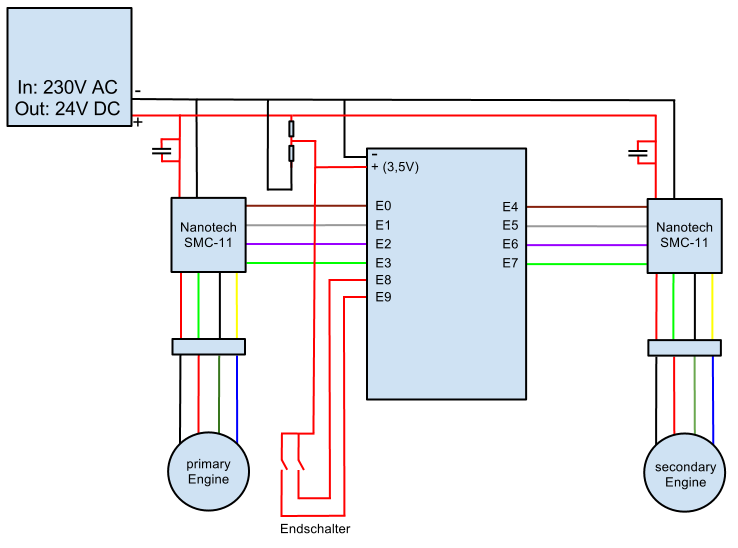
\includegraphics[width=14cm]{images/edubot_electronic} 
    \caption{Schematische Darstellung der Elektronik}
  \end{minipage}
\end{figure}

\subsubsection{Motoren und Steuerungen}
Als Motoren kamen beim Edubot Modell zwei Schrittmotoren der Firma Nanotech zum Einsatz. Die beiden Motoren werden jeweils über eine seperate Schrittmotorsteuerung gesteuert. Die Steuerungen vom Typ Nanotech SMC-11 übernahmen die Stromversorgung, sowie die direkte Ansteuerung der Motoren.

\begin{itemize}
\item \textbf{Steuerung}\\
Aufgabe der beiden Nanotech SMC-11 Steuerungen ist vor allem die direkte Ansteuerung der Motoren. Dazu muss sie über die 4 Verbindungskabel zum Motor Stromimpulse für das verfahren der einzelnen Takte übergeben.
Die beiden Motorsteuerungen verfügen jeweils über 4 Digitale Eingänge über die bestimmt wann der Motor einen Schritt fahren soll, in welche Richtung der Schritt durchgeführt werden soll, ob der Motor Ein- oder Ausgeschaltet ist und ob die Automatische Spannungsabsenkung (reduziert die Aufgenommene Leistung bei Stillstand des Motors nach 3 Sekunden automatisch um die Motorspulen zu schonen).
Die genannten Eingänge sind mit Ausgabeports des Mikrocontrollers verbunden, damit übernimmt der Mikrocontroller die Übergabe der Parameter.

\item \textbf{Motoren}\\
Da es sich bei den beiden Motoren des Typs Nanotech ST2818L1006-1 um bipolare Schrittmotoren handelt ermöglichen sie die Einteilung einer ganzen Umdrehung in eine bestimmte Anzahl an Schritten. Bipolar bedeutet das die Ansteuerung des Motors komplexer ist, dafür mehr Leistung abverlangt werden kann, die Steuerung muss hierzu den bipolaren Betrieb des Motors unterstützen.
In diesem Projekt wurde außerdem der 16 fache Mikroschrittmodus gewählt, dies ermöglicht die Teilung der einzelnen Schritte des Motors in Teilschritte um damit eine höhere Genauigkeit zu erreichen. Der Spezifikation der Motoren ist zu entnehmen, dass ein Vollschritt 1,8$^\circ$ hat, ein Mikroschritt wie er bei unseren Verfahrbeweungen verwendet wird sind also 0,1125$^\circ$. 

\item \textbf{Endschalter}\\
Um den Roboter in seine Ausgangsposition fahren zu können muss er zuerst an die Grenzen seines Arbeitsbereichs fahren, von dort aus weiß der Mikrocontroller welche Winkel die einzelnen Motoren fahren müssen um in die Ausgangsposition zu kommen.
Damit der erkannt werden kann wann die Grenzen des Arbeitsbereichs erreicht sind, wurden zwei Endschalter in Form von einfachen Kontaktstellen an den beiden Achsen und an der Basis angebracht. Stößt der Arm nun im Rahmen des Homings (Finden der Ausgangsposition) an die Basis, bzw. erreicht die zweite Achse ihren Maximalwinkel, so wird ein Kontakt hergestellt und der Mikrocontroller empfängt an einem Digitalen Eingang ein Signal. Realisiert wurden die Kontaktstellen als einfache Flächen aus Stahl, wobei auf die Verwendung vorgefertigter mechanischer Endschalter bewusst verzichtet wurde um Probleme mit dem Druckpunkt zu vermeiden.
\end{itemize}


